\chapter{Day 5: arrays}

\section{Summary of topics}
% Summarize the topics from the “listen” segment of the day (150 – 250 words)

The topic of today were arrays. Arrays store a set of data elements under the same name. They can store all sorts of data types, but only one at the same time. They are especially useful for storing related data together, so you don't need to create lots of separate variables. There are a few different ways to create an array

\begin{codebox}{Example 5.1}
    \begin{lstlisting}
int[] data; // declare
data = new int[5]; // initialize 
data[0] = 10; // assign

int[] data = new int[5]; // declare, initialize
data[0] = 0; // assign

int[] data = {10, 5, 7, 12, 20}; // initialize, declare, assign
    \end{lstlisting}
\end{codebox}

You create an array using the datatype followed by square brackets and the variable name. Then, you can either use \texttt{new datatype[n]} to create an array of size \texttt{n} or use curly brackets followed by a number of variables separated by commas to immediately fill the array.

You can read a write data from the array by typing its name followed by square brackets. Inside these brackets you type the index of the value you want to get. The index is the position of the data in the array, starting at 0 for the first elements. You can write to an array by using the same method as before, together with the assign operator and the (new) value you want in the array. See example 5.2

\begin{codebox}{Example 5.2}
    \begin{lstlisting}
int[] data = {10, 5, 7, 12, 20};

data[3] // this will give the fourth value, 12
data[0] = 15; // set the first value (10) to 15
    \end{lstlisting}
\end{codebox}

important to note that if the index is not in the array (like -1 or in the example, 5), you get an error.

\newpage

The final topic was how you can use arrays in loops. Example 5.3 was shown during the lesson.

\begin{codebox}{Example 5.2}
    \begin{lstlisting}
float[] grades = {6, 6.5, 9, 8.5, 5};
float total = 0;

for(int i = 0; i < grades.length; i++){
    total += grades[i];
} 
println(total/grades.length);
    \end{lstlisting}
\end{codebox}

This code creates an array of grades and a variable \texttt{total} that will be used to store the sum of the grades. In a for loop the variable \texttt{i} starts at 0 and increases every iteration by 1. \texttt{grades.length} gets the length of the array, so the loop stops at the end of the array. Inside the loop, each value of the array is added to the \texttt{total} variable, which results in this variable being equal to the sum of the values in \texttt{grades}. Outside of the loop the average of the grades is printed. 

\section{Challenge description: Tetris}
% A description of that day’s challenge describing what the assignment was, what you tried to achieve and how you applied the topics from the “listen” segment. include instruction on how to use is and Include screenshots/screen captures. (150 – 250 words)

My intention for this final challenge was to create the classic game Tetris, for this I wanted to recreate in faithfully to the classic GameBoy version of the game. Just like the original, I wanted the game to randomly give the player one of the seven Tetris blocks, which slowly starts moving down the screen. The player can move the block left and right, and also rotate the block or move it down more quickly. Once the block is placed and a full row is created, the row should be removed and all the rows should shift down. Finally, the game should award points to the player and give the player a new random block. If this proved to be easy, I also wanted to recreate the look of the game, add the possibility to save a highscore and add a simple menu to the game. The original version is shown in \cref{fig: tetris gb}.

\begin{figure}[H]
    \centering
    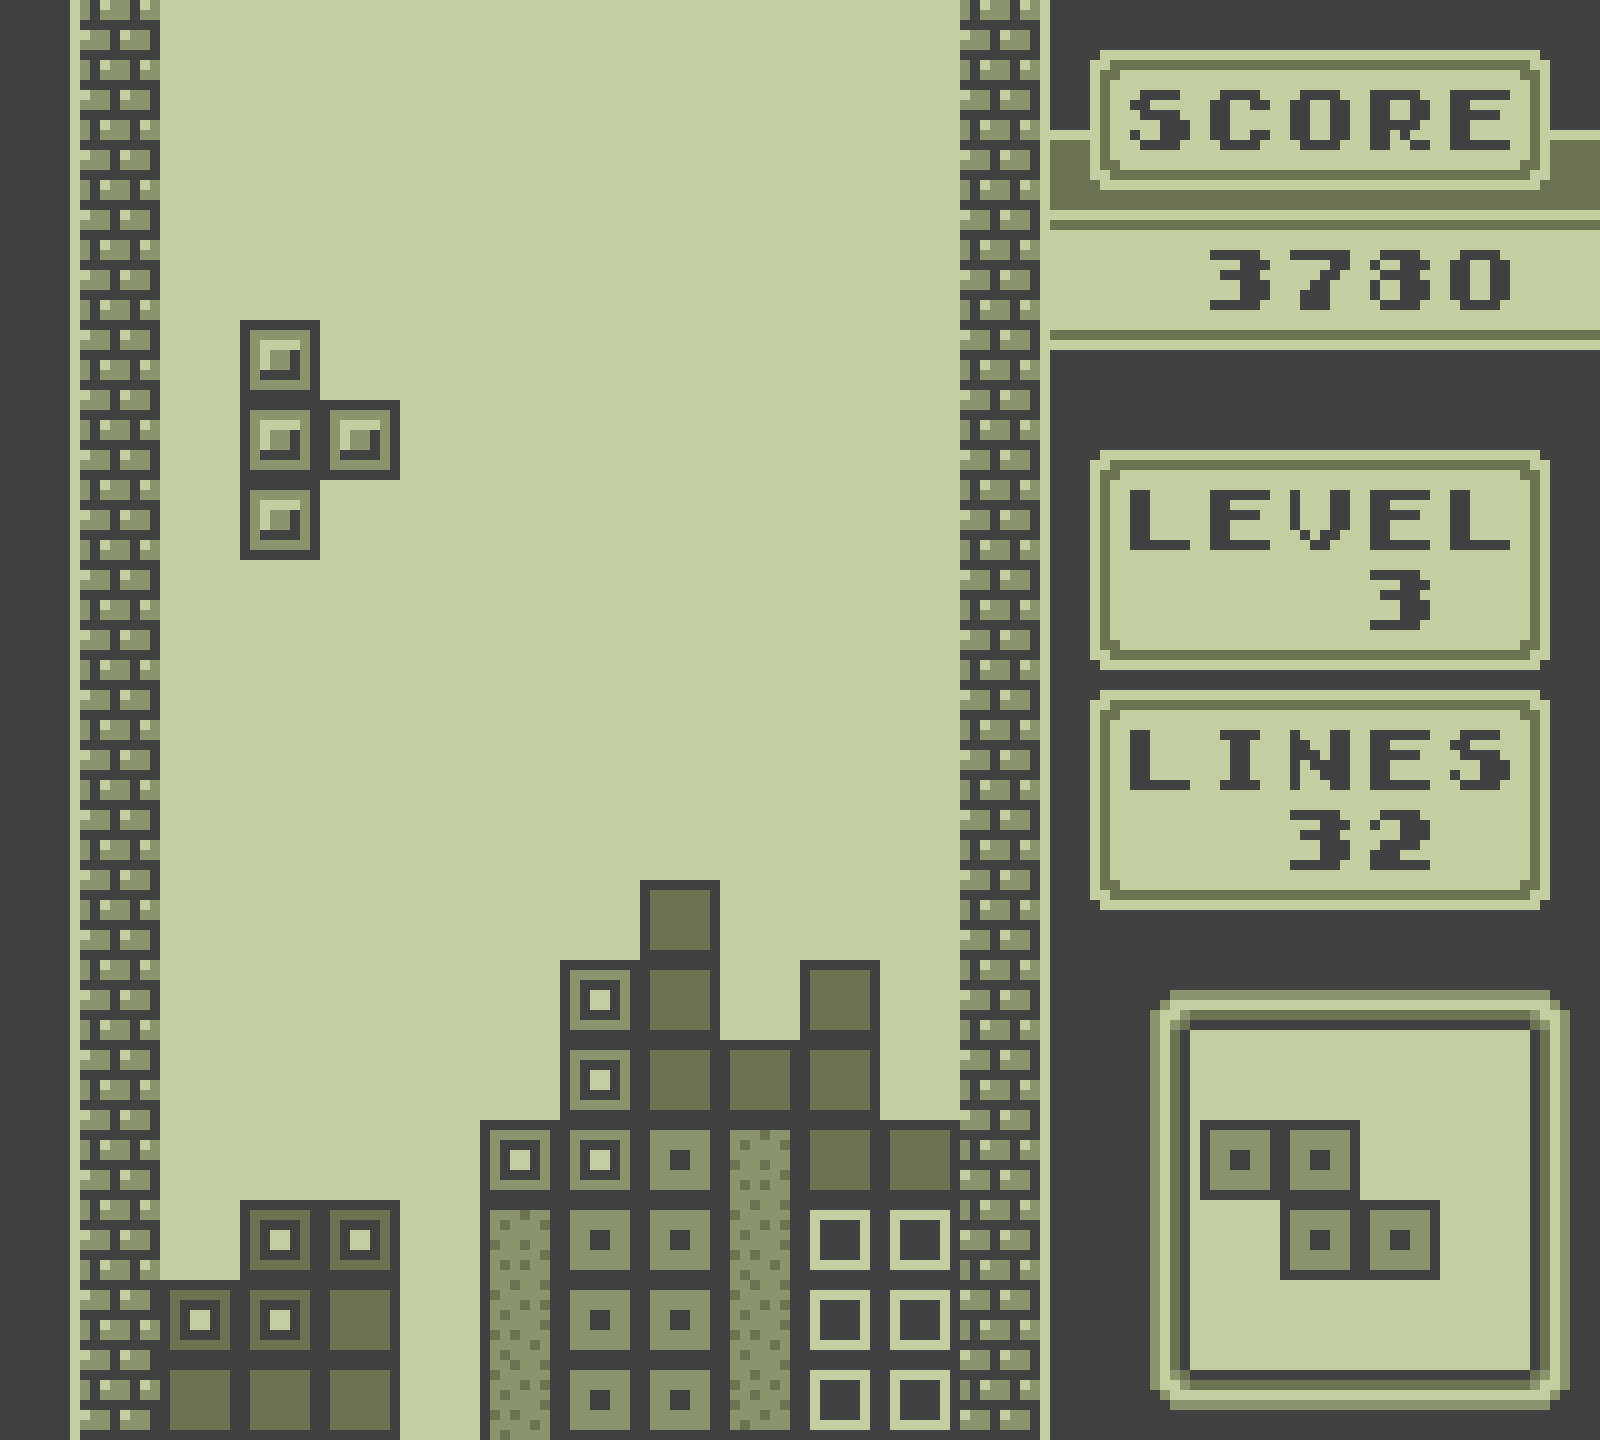
\includegraphics[width = 0.5 \textwidth]{Figures/day_5/gb_tetris.png}
    \caption{The original Tetris for the GameBoy}
    \label{fig: tetris gb}
\end{figure}

In \cref{fig: tetris}. It is shown how a typical game is played. When launching the game a start screen is shown with the current highscore. You can press the enter-key to start the game (\cref{fig: new game}). The game is played using the arrow keys, where the left and right keys move the block left and right. Pressing and holding the down key moves the block down more quickly. The up key rotates the pieces (\cref{fig: game}). The goal is to create a full line of blocks after which that row is removed from the playing field. The number of points scored are based on the current level and the number of lines cleared at the same time. Every 5 cleared lines the level is increased to a maximum of 12. The speed of the game will increase each level. One can pause and unpause the game at any moment by pressing the enter key (\cref{fig: paused game}). The game is over when a new block cannot be created. The score and highscore are shown and one can press the enter key again to go back to the main menu (\cref{fig: game over}). 

\begin{figure}[H]
    \centering
    \begin{subfigure}[b]{0.35\textwidth}
        \centering
        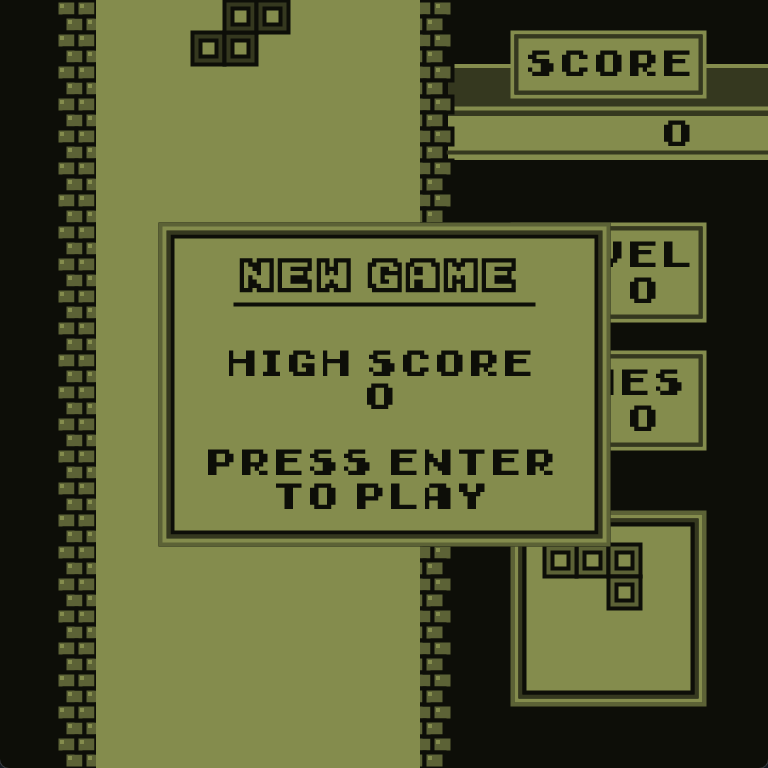
\includegraphics[width=\textwidth]{Figures/day_5/new_game.png}
        \caption{Starting a new game}
        \label{fig: new game}
    \end{subfigure}
    \hspace{1cm}
    \begin{subfigure}[b]{0.35\textwidth}
        \centering
        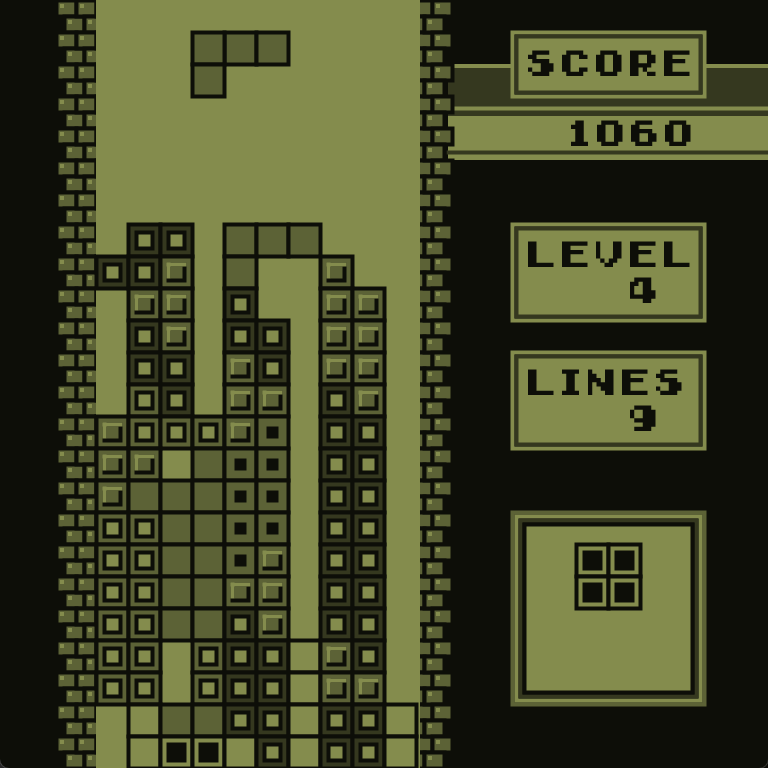
\includegraphics[width=\textwidth]{Figures/day_5/game.png}
        \caption{Playing te game}
        \label{fig: game}
    \end{subfigure}
    \begin{subfigure}[b]{0.35\textwidth}
        \centering
        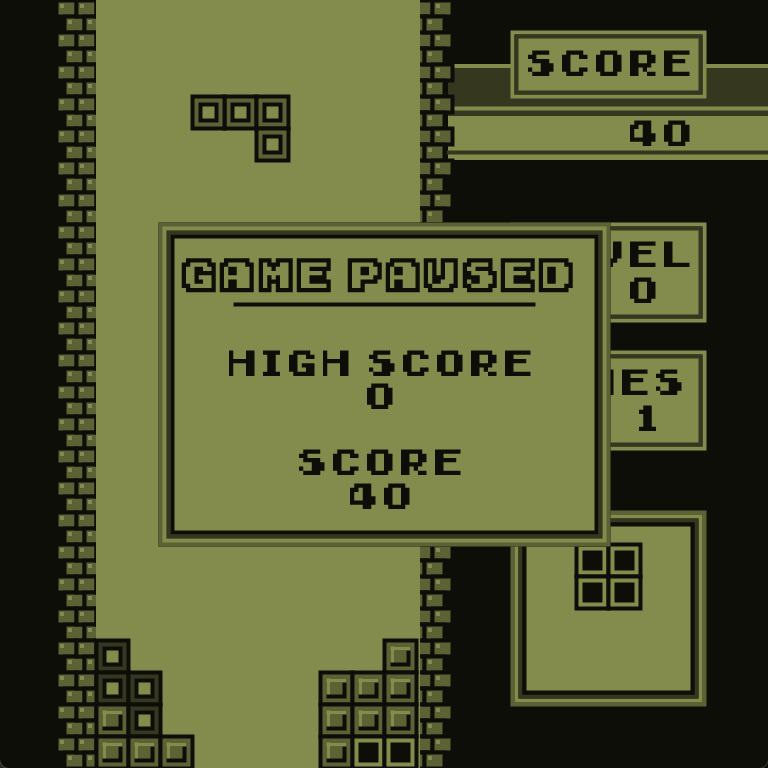
\includegraphics[width=\textwidth]{Figures/day_5/game_paused.png}
        \caption{Pausing the game}
        \label{fig: paused game}
    \end{subfigure}
    \hspace{1cm}
    \begin{subfigure}[b]{0.35\textwidth}
        \centering
        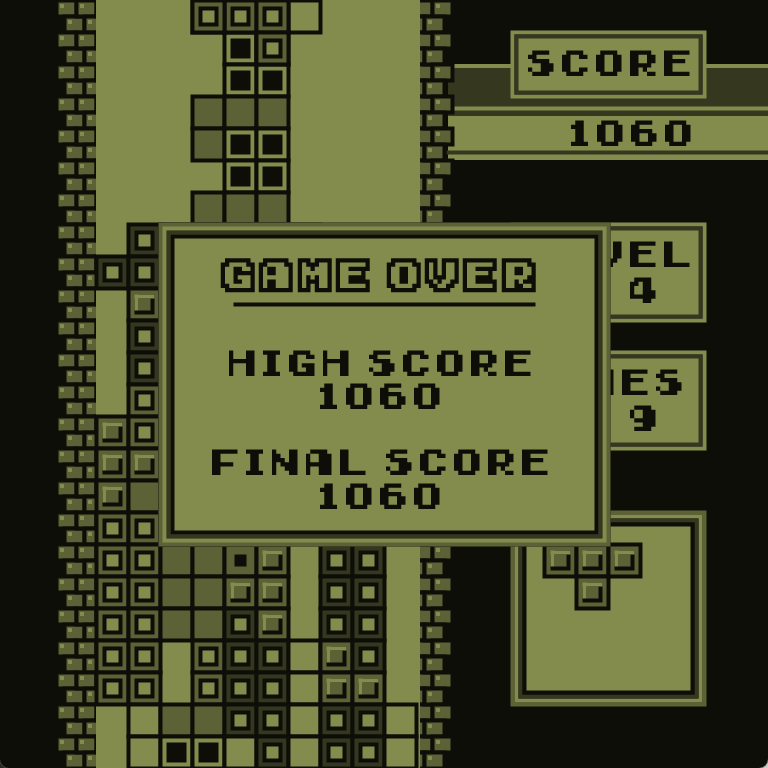
\includegraphics[width=\textwidth]{Figures/day_5/game_over.png}
        \caption{Game over}
        \label{fig: game over}
    \end{subfigure}

    \caption{A typical game of Tetris}
    \label{fig: tetris}

\end{figure}